\subsubsection{25.11.14}

\begin{enumerate}
	\item Время начала и окончания собрания:
	17:00 - 21:00
	\item Цели собрания:
	\begin{enumerate}
		\item Распутать провода и провести их наиболее аккуратным способом.
		
		\item Увеличить количество приводов, отвечающих за приведение в движение лебедки с двух до четырех.
		
		\item Убрать передаточное отношение с механизма лебедки.
		
	\end{enumerate}
	\item Проделанная работа:
	\begin{enumerate}
		\item Проводка была переделана таким образом, чтобы провода не путались, не занимали внутри робота много места и не мешали замене аккумулятора.
		
		\begin{figure}[H]
			\begin{minipage}[h]{0.2\linewidth}
				\center  
			\end{minipage}
			\begin{minipage}[h]{0.6\linewidth}
				\center{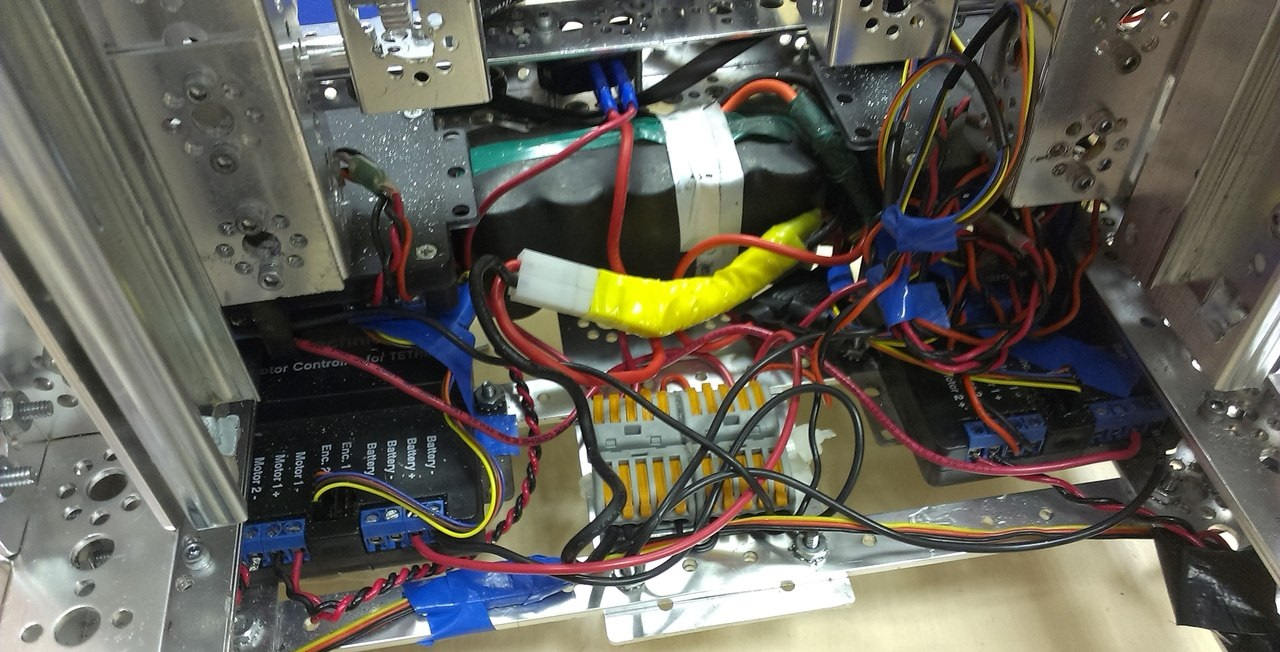
\includegraphics[scale=0.2]{days/25.11.14/images/01}}
				\caption{Внутреннее пространство робота после оптимизации проводки}
			\end{minipage}
		\end{figure}
		
		\item Была начата переделка механизма лебедки под четыре привода.
		
		\item Поскольку мы добавили в конструкцию два дополнительных привода, нам понадобилось установить еще один драйвер приводов для управления ими. Он был установлен вместо драйвера сервоприводов внутрь корпуса робота, а драйвер сервоприводов было перемещен в более доступное место, поскольку так будет удобнее подключать к нему новые сервоприводы, если у нас появится в этом необходимость.
		
		\item Все четыре драйвера были подключены к 1-му входу NXT-блока, а драйвер сервоприводов - ко 2-му. В соответствии с этим, инициализация приводов и сервоприводов во всех программах была изменена.
		
		\begin{figure}[H]
			\begin{minipage}[h]{0.2\linewidth}
				\center  
			\end{minipage}
			\begin{minipage}[h]{0.6\linewidth}
				\center{
\includegraphics[scale=0.2]{days/25.11.14/images/02}}
				\caption{Драйвер сервоприводов}
			\end{minipage}
		\end{figure}
		
	\end{enumerate}
	
	\item Итоги собрания: 
	\begin{enumerate}
		\item Проводка оптимизирована.
		
		\item Драйвер приводов установлен.
		
		\item Драйвер сервоприводов перемещен в более доступное место.
		
		\item Переделка механизма лебедки начата.
		
	\end{enumerate}
	
	\item Задачи для последующих собраний:
	\begin{enumerate}
		\item Завершить изменение механизма лебедки.
		
		\item Разработать концепцию нового механизма захвата мячей.
		
	\end{enumerate}     
\end{enumerate}
\fillpage